In this lab we use bootable tools with write-blocking technologies to gather data from a system without compromising the original system.

\section*{2: Applied Learning}

\subsection*{Part 1: Explore a Windows Workstation with Helix}

In this section we use the Helix forensic investigation tool to identify specific data items such as disk information and image data.

\begin{figure}[H]
    \centering
    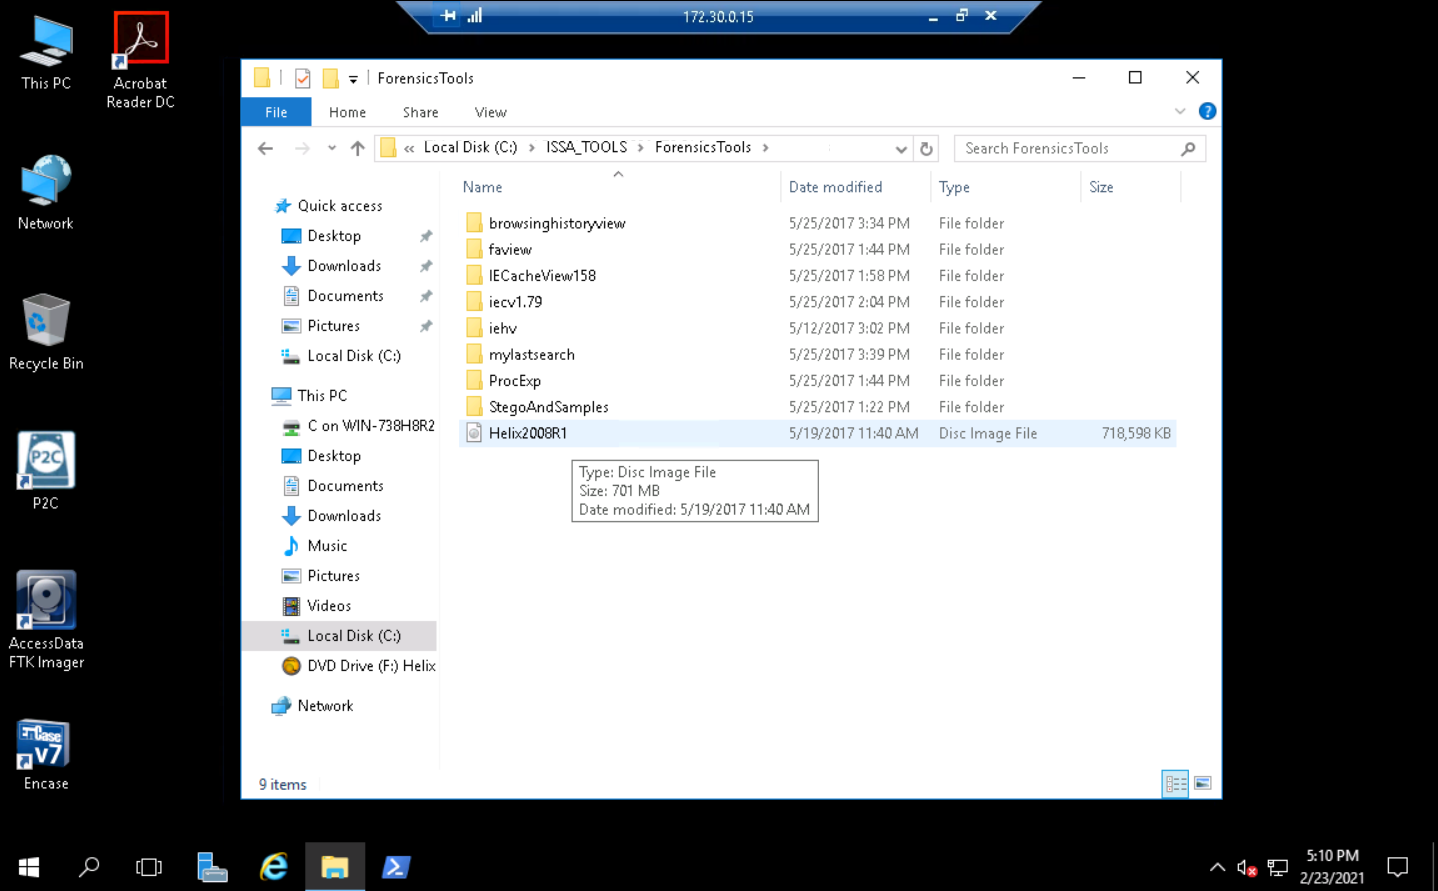
\includegraphics[width=\linewidth]{figures/Part 1 Step 2.png}
    \caption{Helix application welcome screen.}
\end{figure}

\begin{figure}[H]
    \centering
    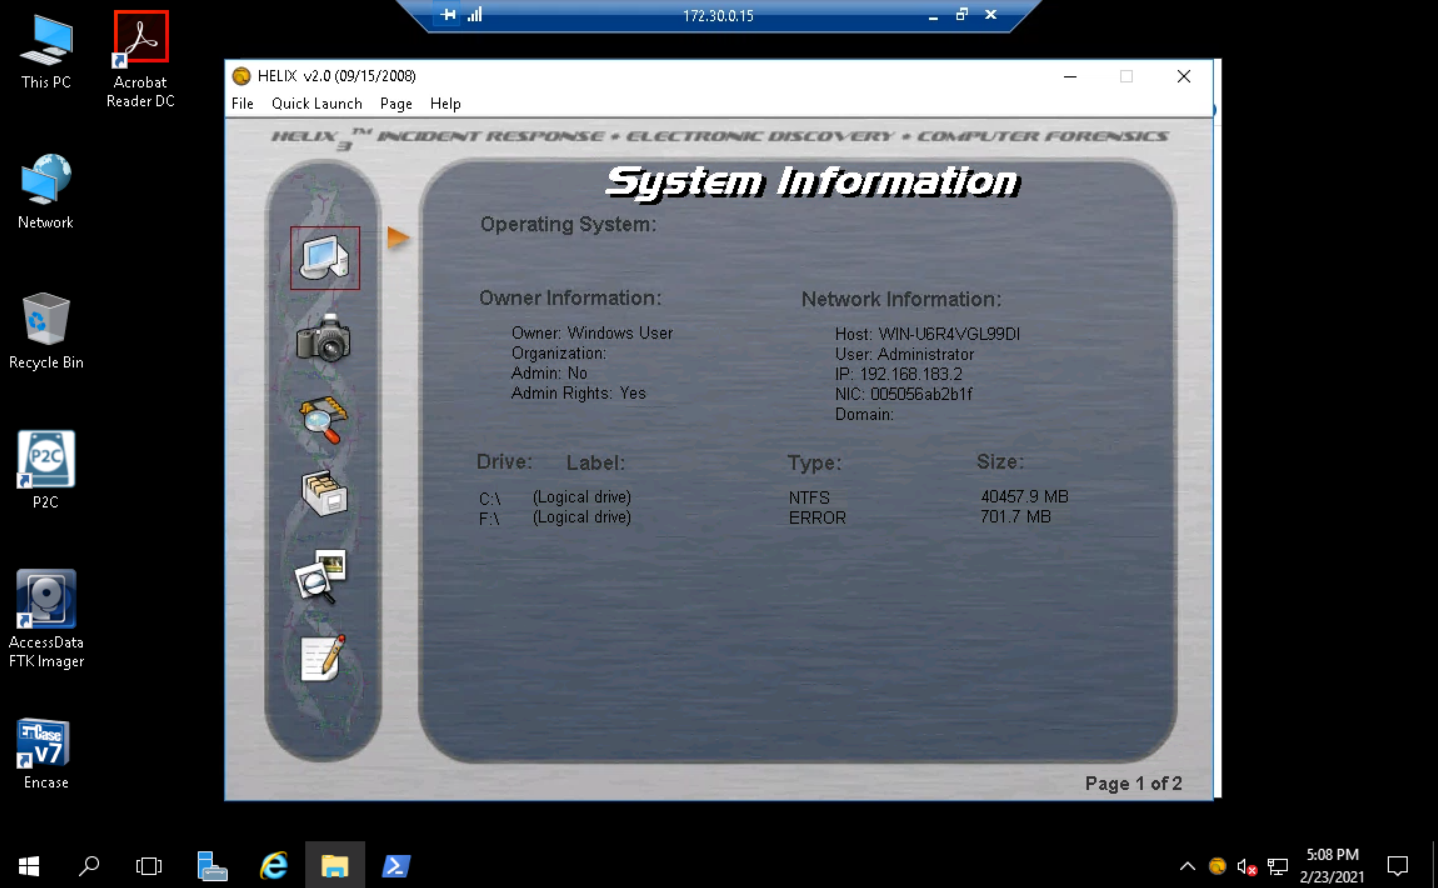
\includegraphics[width=\linewidth]{figures/Part 1 Step 4.png}
    \caption{Network information on Preview System Information page.}
\end{figure}

\begin{figure}[H]
    \centering
    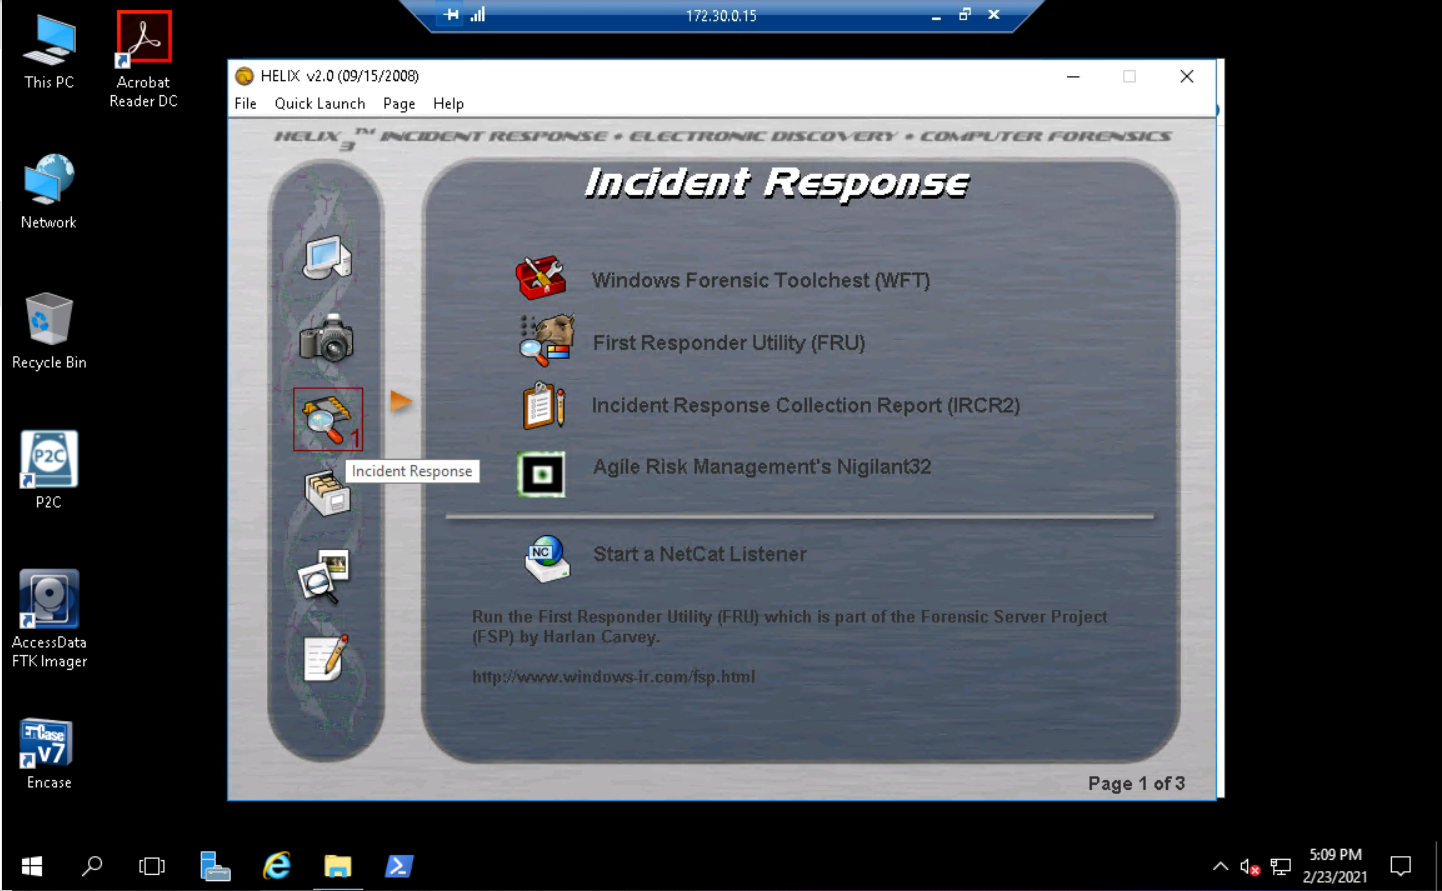
\includegraphics[width=\linewidth]{figures/Part 1 Step 5.png}
    \caption{Incident response tools for Windows Systems.}
\end{figure}

\begin{figure}[H]
    \centering
    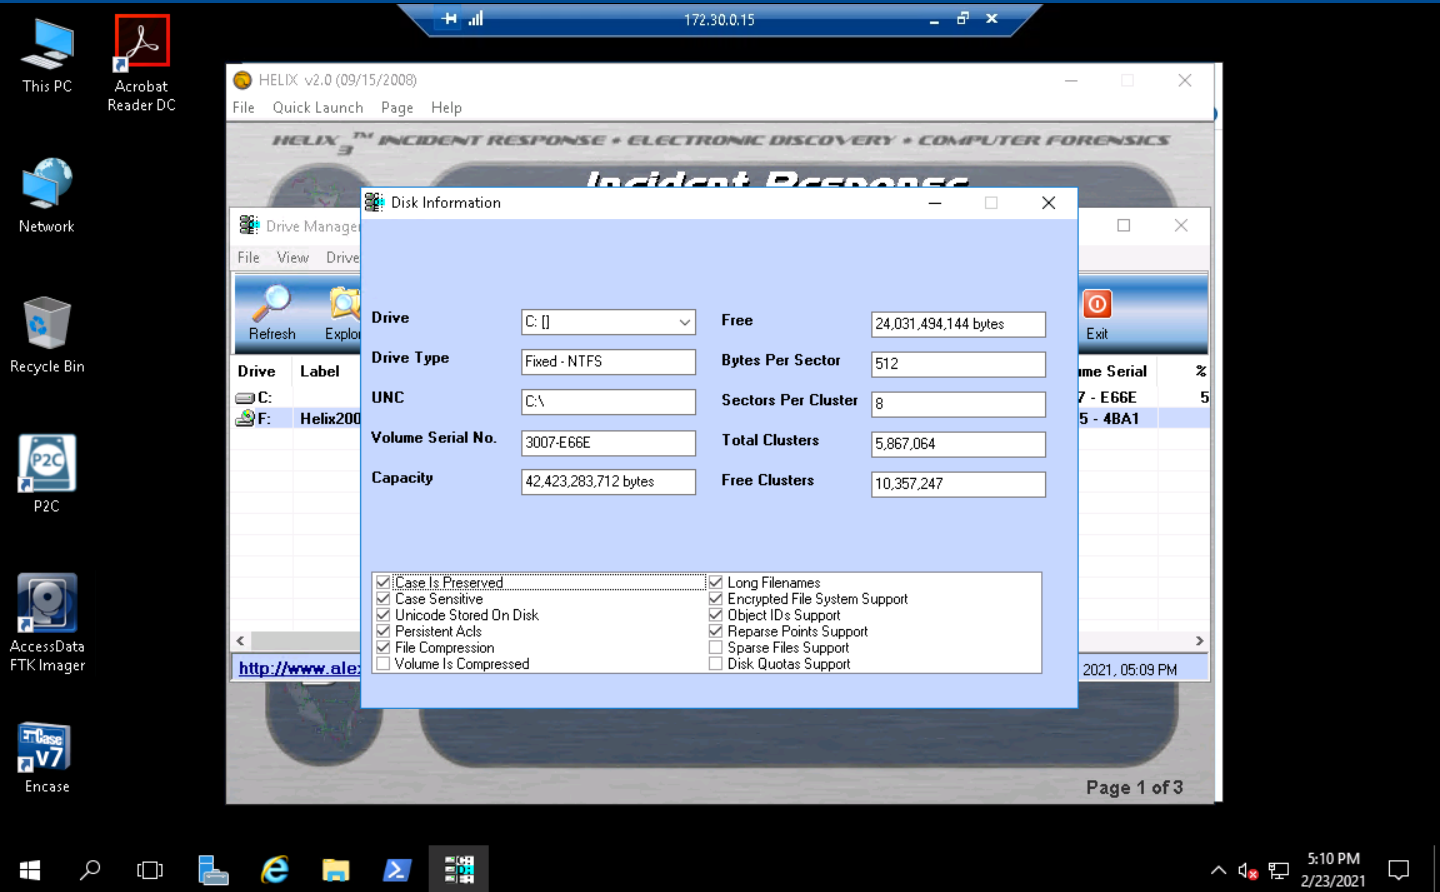
\includegraphics[width=\linewidth]{figures/Part 1 Step 8.png}
    \caption{Disk information for the {\tt C:} drive.}
\end{figure}

\begin{figure}[H]
    \centering
    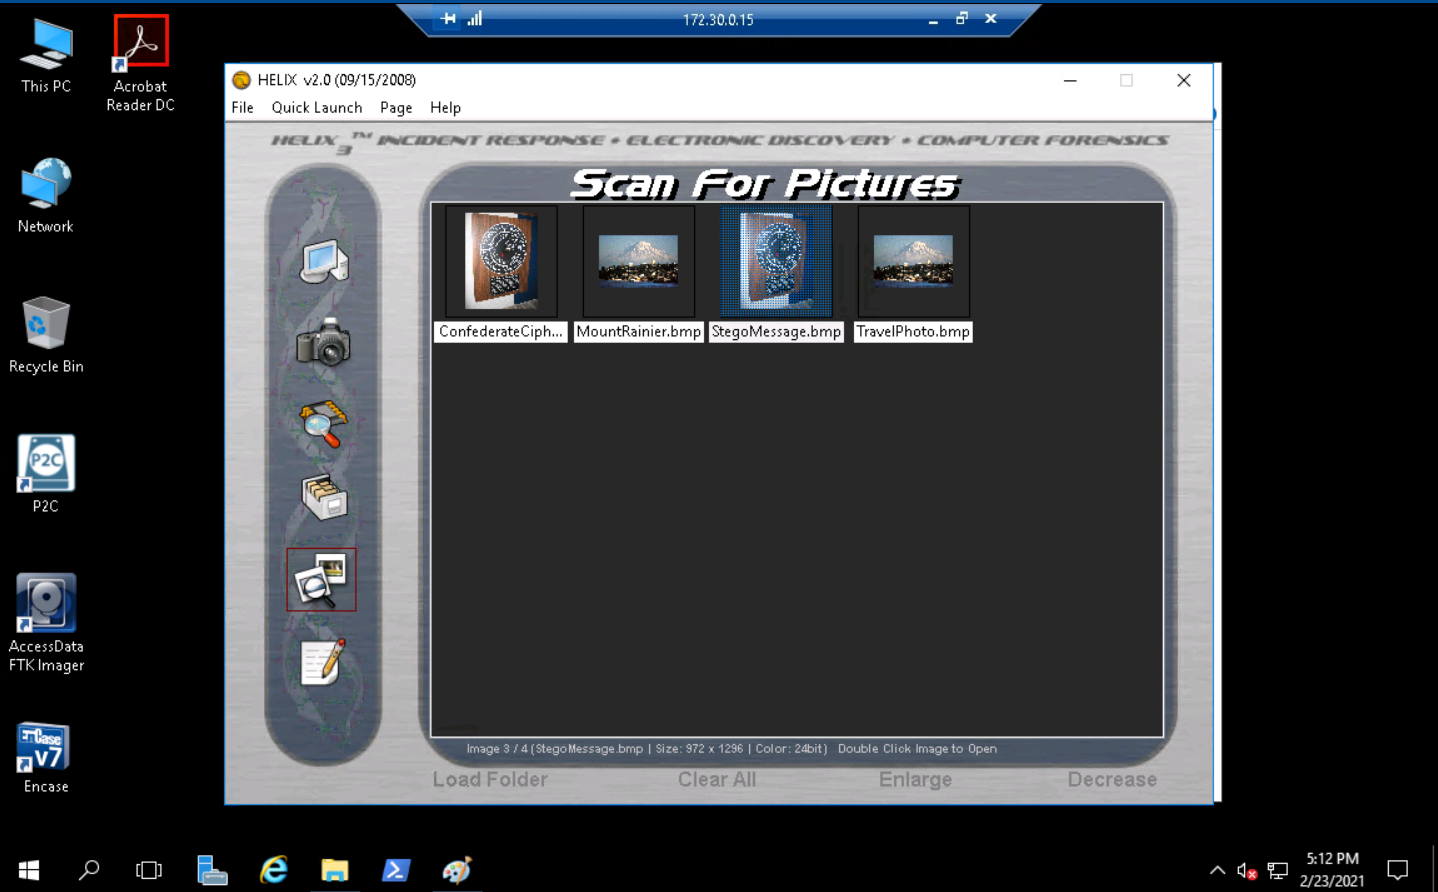
\includegraphics[width=\linewidth]{figures/Part 1 Step 11.png}
    \caption{StegoAndSamples folder.}
\end{figure}

\begin{figure}[H]
    \centering
    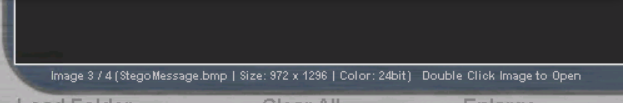
\includegraphics[width=\linewidth]{figures/Part 1 Step 13.png}
    \caption{Data points associated with the image.}
\end{figure}

\begin{figure}[H]
    \centering
    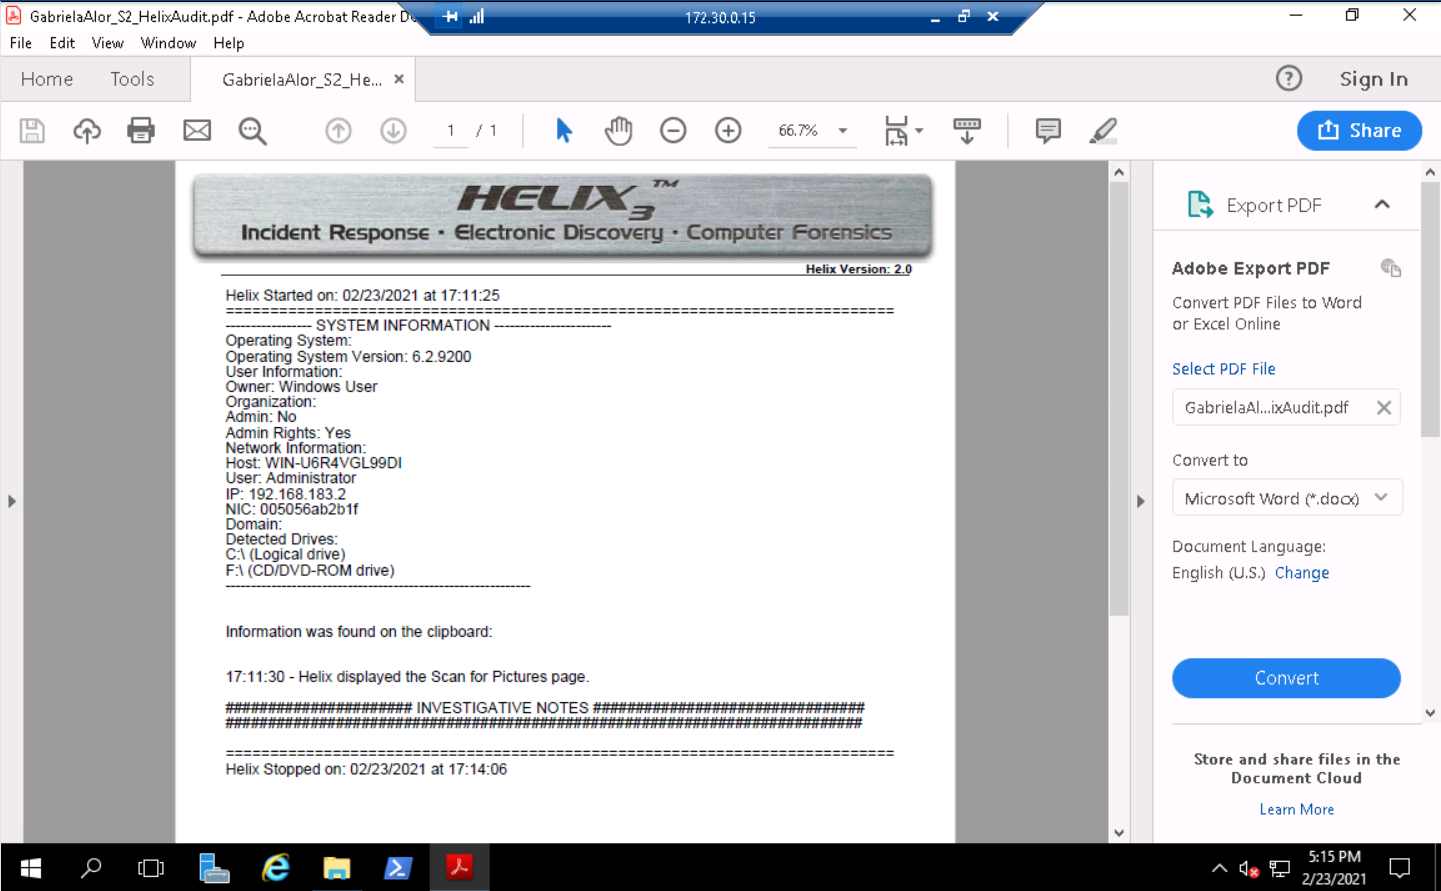
\includegraphics[width=\linewidth]{figures/Part 1 Step 14.png}
    \caption{Helix audit log.}
\end{figure}

\section*{Part 2: Forensic Tools to Extract Data}
In this section we remotely connect to a Windows machine and extract data from the Internet Explorer browser using multiple forensic tools.

The process explorer is similar to the Windows task manager, but displays much more data than 
\begin{figure}[H]
    \centering
    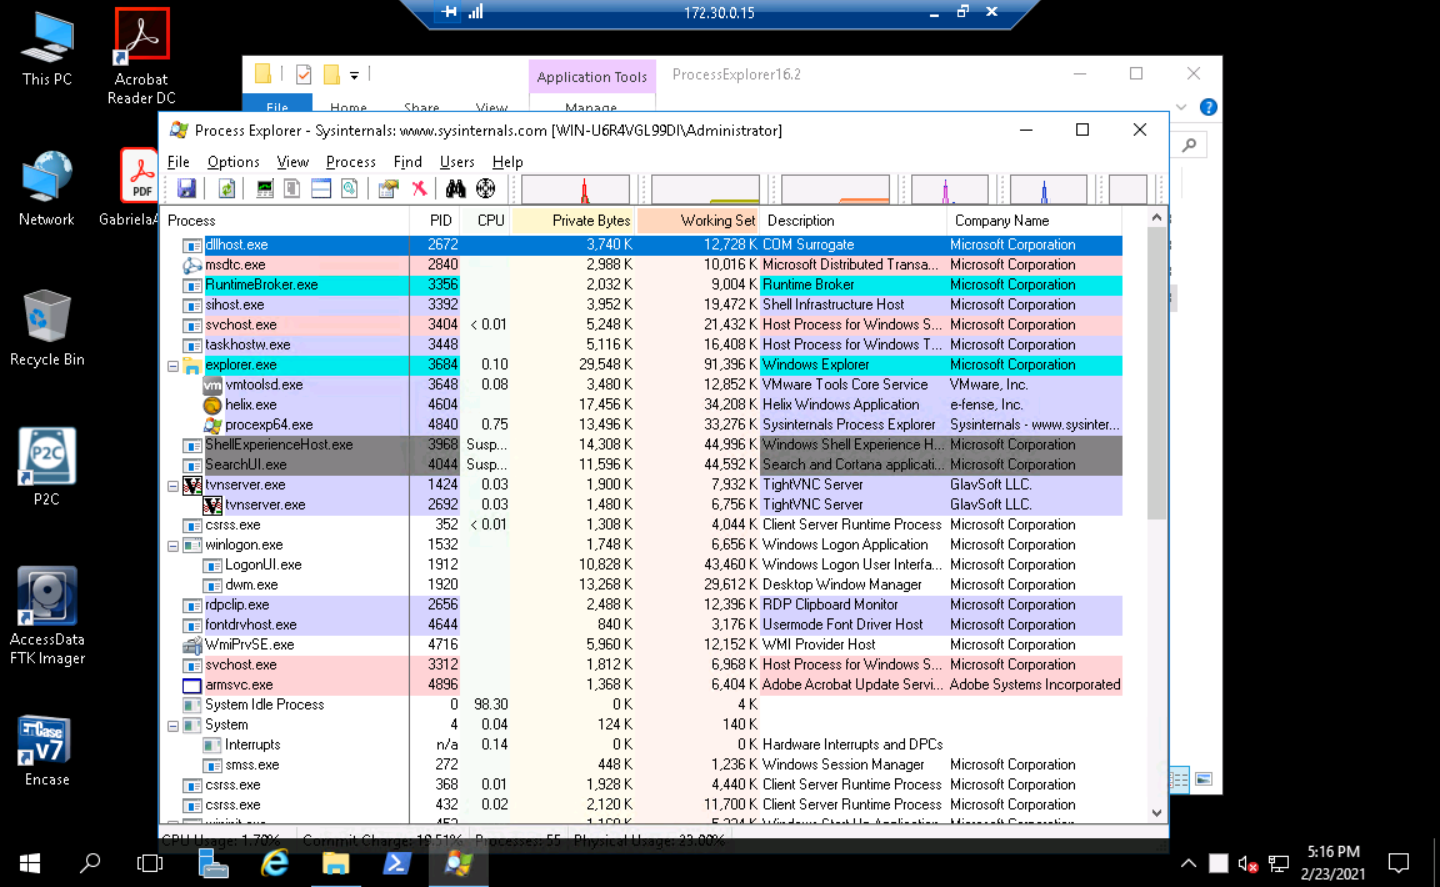
\includegraphics[width=\linewidth]{figures/Part 2 Step 1.png}
    \caption{ProcessExplorer16.2}
\end{figure}

\begin{figure}[H]
    \centering
    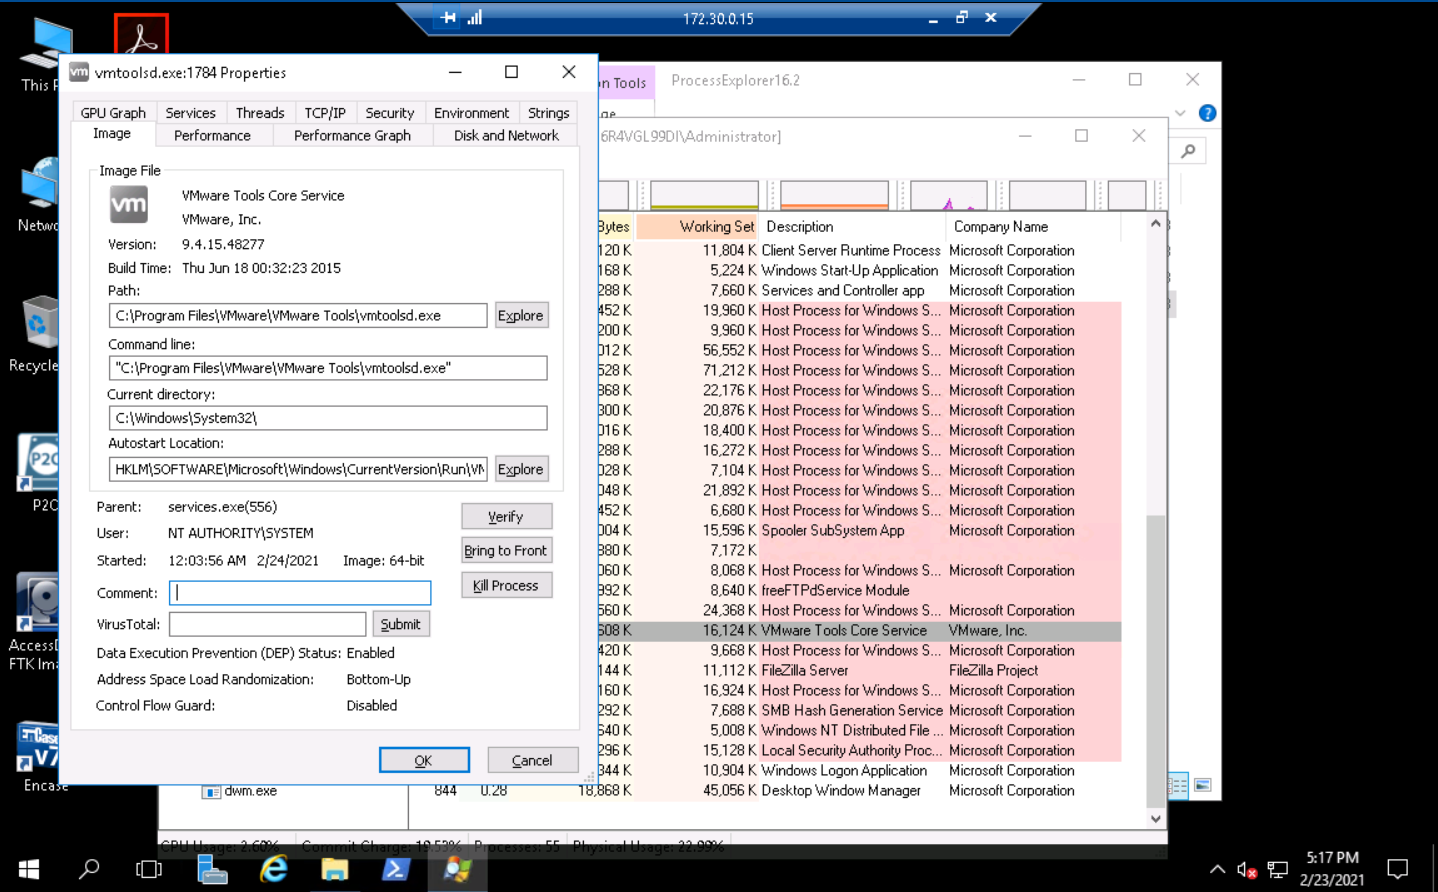
\includegraphics[width=\linewidth]{figures/Part 2 Step 3 Image.png}
    \caption{vmtools.exe process Image tab.}
\end{figure}

\begin{figure}[H]
    \centering
    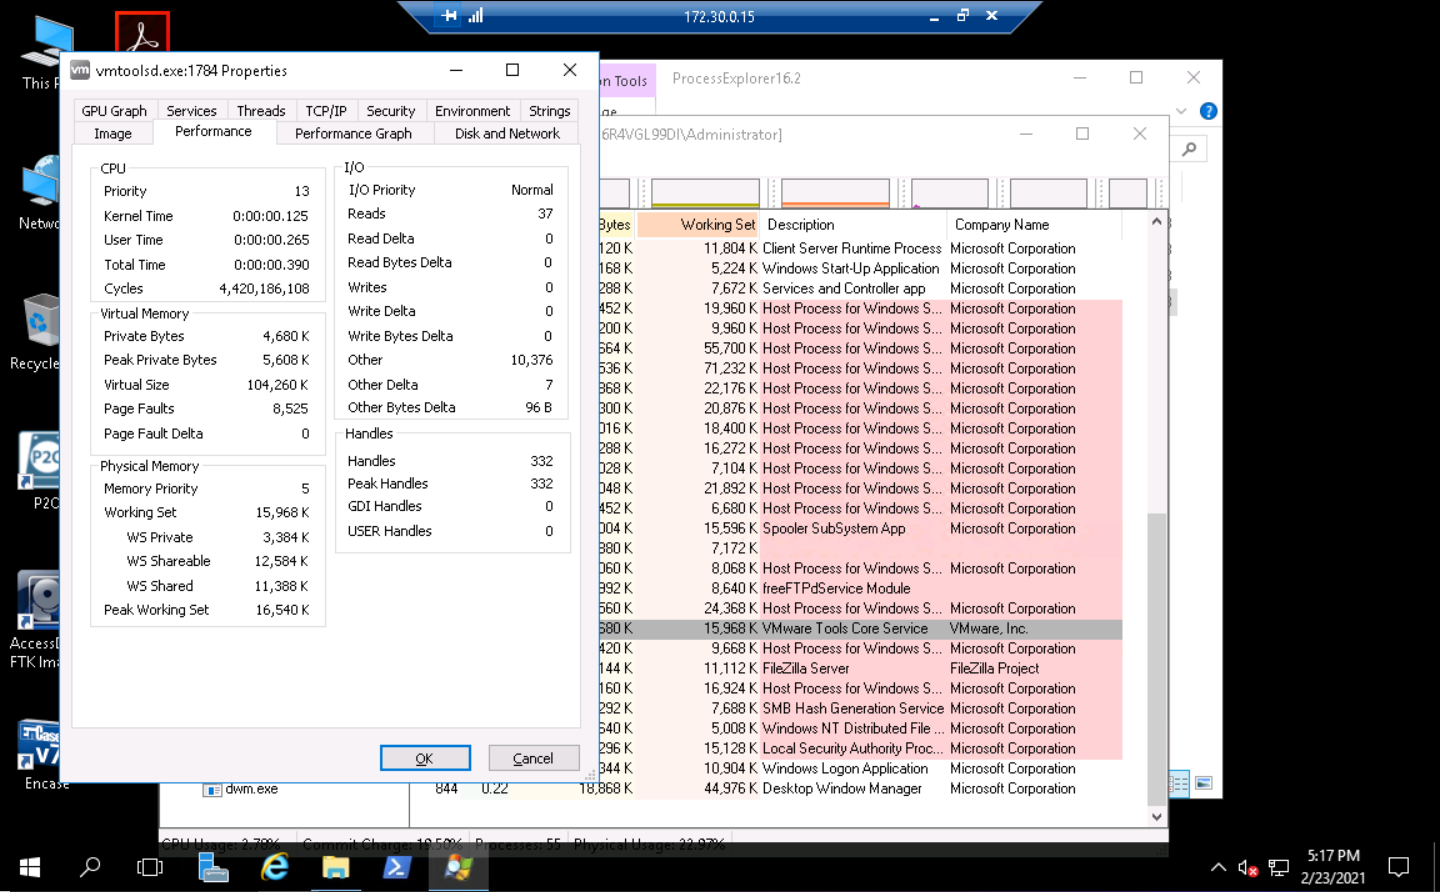
\includegraphics[width=\linewidth]{figures/Part 2 Step 3 Performance.png}
    \caption{vmtools.exe process Performance tab.}
\end{figure}

FavoritesView summarizes all bookmarks and favorites saved from  browsers, and allows you to view them in its own browser.
\begin{figure}[H]
    \centering
    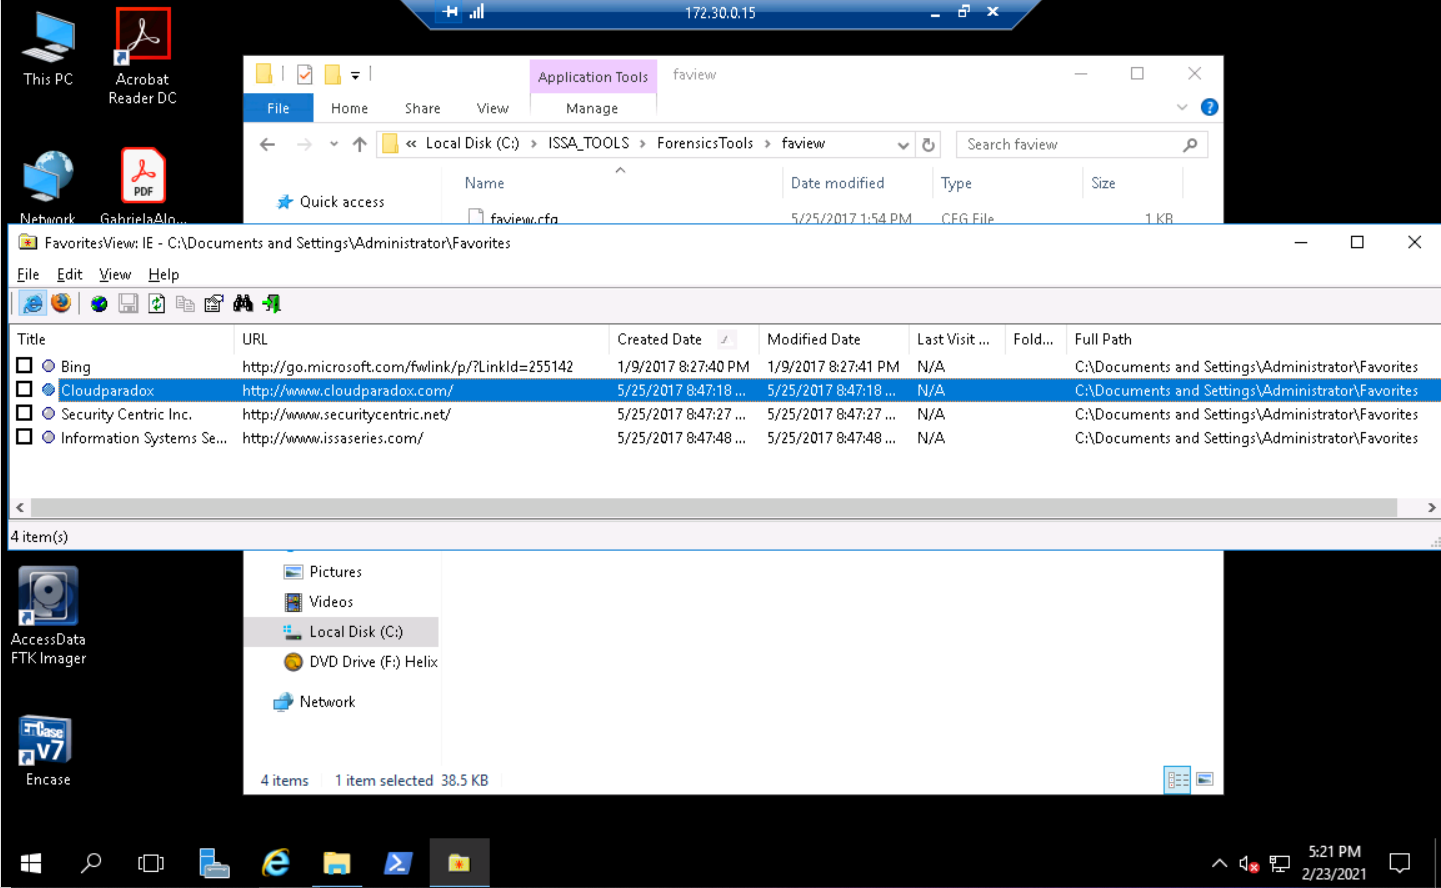
\includegraphics[width=\linewidth]{figures/Part 2 Step 6.png}
    \caption{Faview application.}
\end{figure}

\begin{figure}[H]
    \centering
    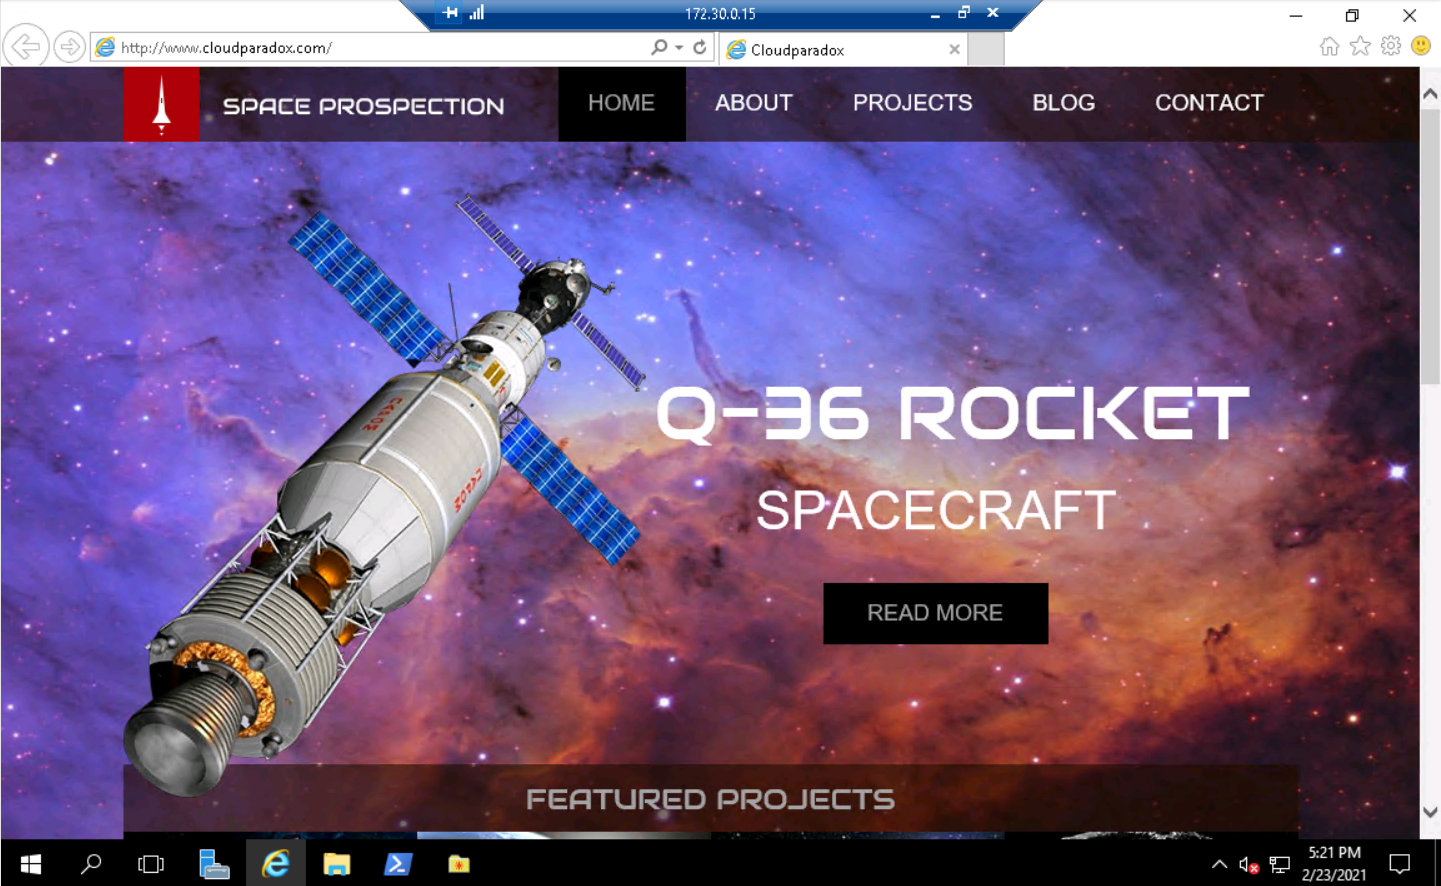
\includegraphics[width=\linewidth]{figures/Part 2 Step 8.png}
    \caption{Cloudparadox web site.}
\end{figure}

IECacheView displays Internet Explorer's cache folder for any user logged onto the local machine and lists all currently stored file types without looking at cookies.
\begin{figure}[H]
    \centering
    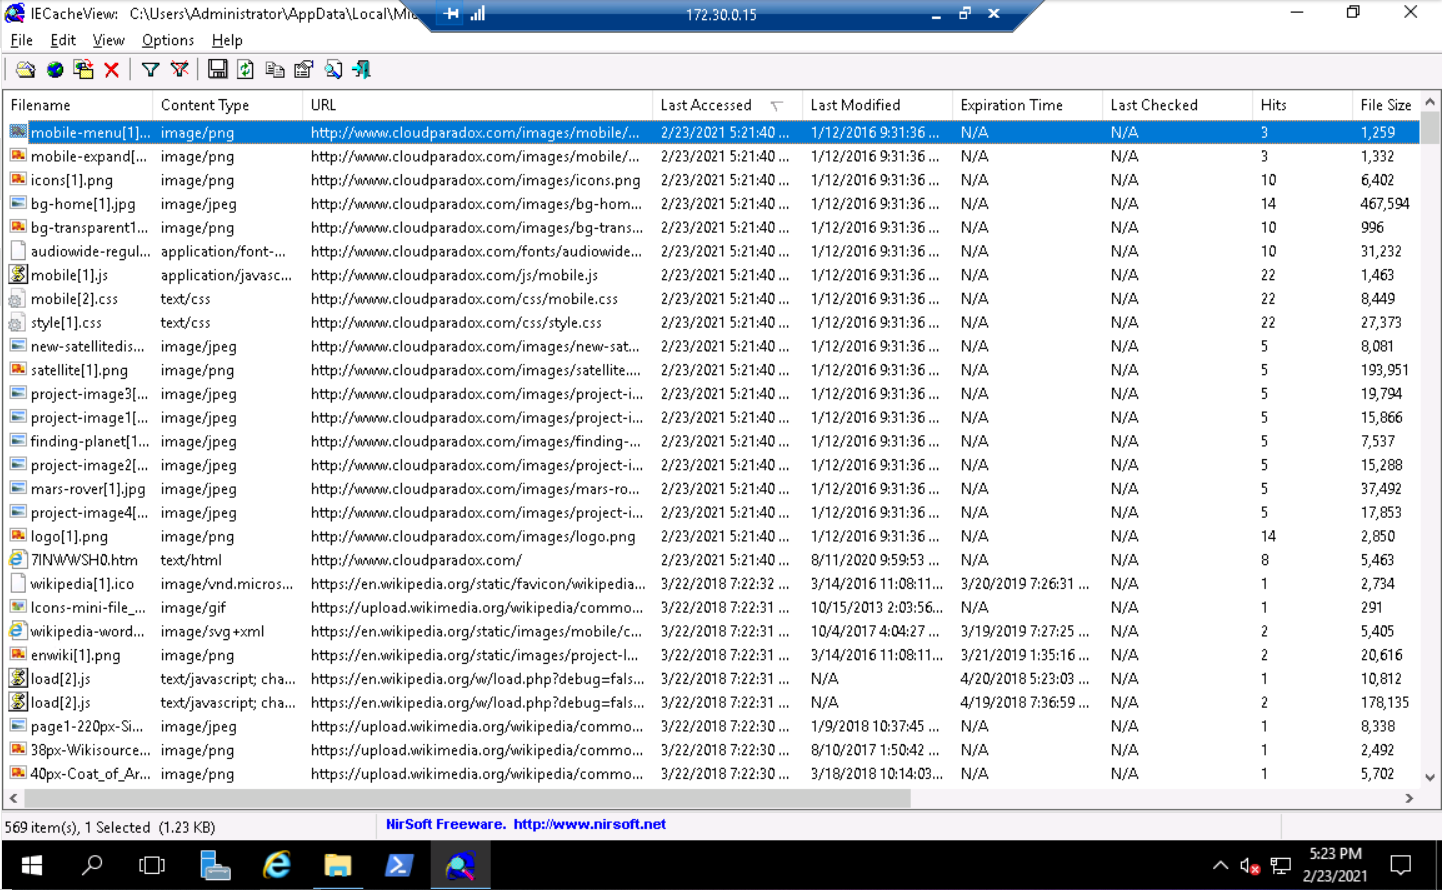
\includegraphics[width=\linewidth]{figures/Part 2 Step 11.png}
    \caption{Most recently accessed item.}
\end{figure}

\begin{figure}[H]
    \centering
    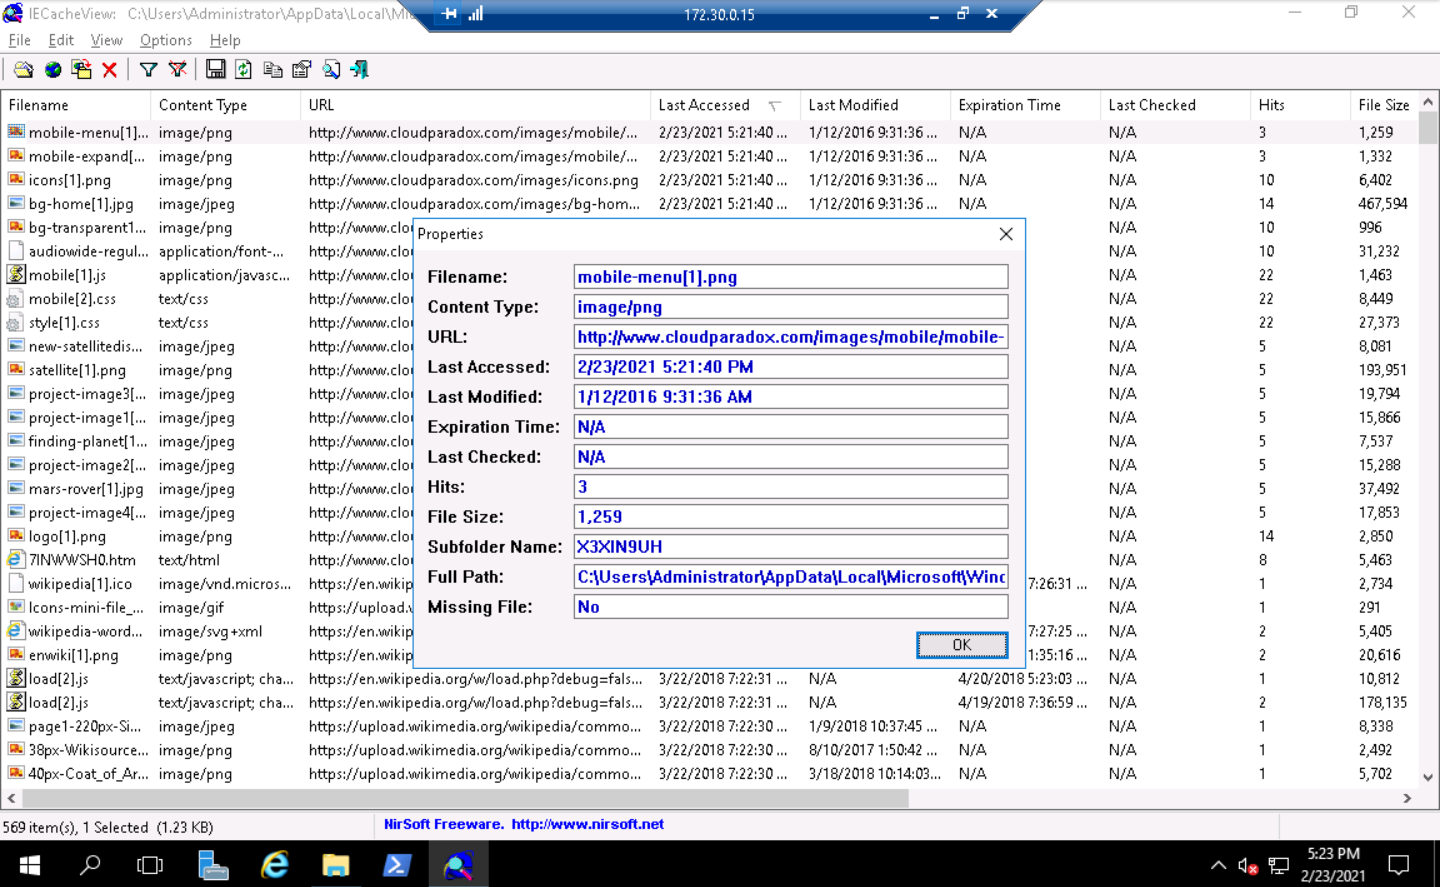
\includegraphics[width=\linewidth]{figures/Part 2 Step 12.png}
    \caption{Properties dialog of the most recently accessed item.}
\end{figure}

\begin{figure}[H]
    \centering
    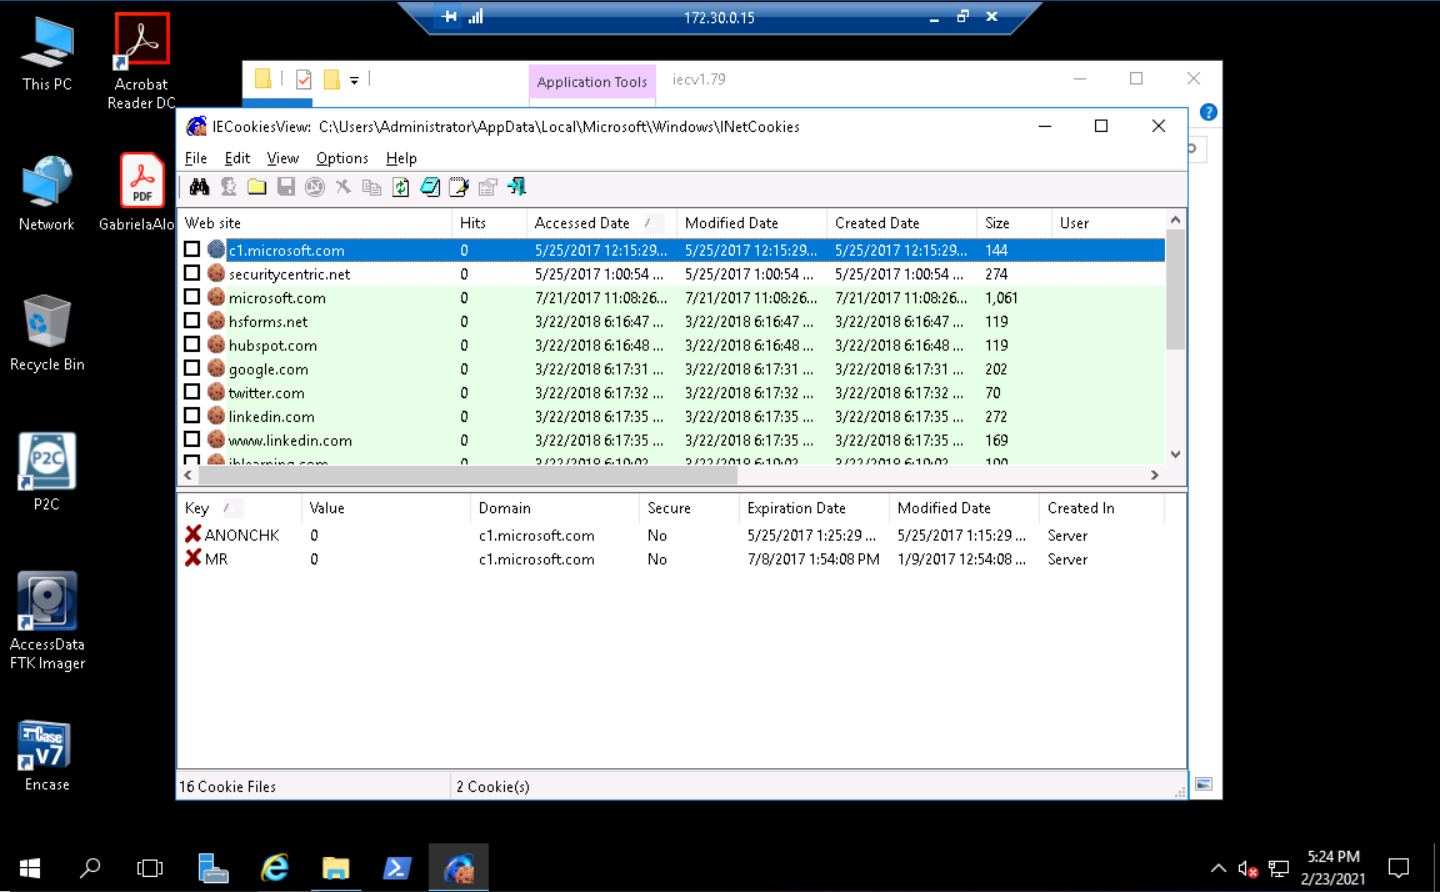
\includegraphics[width=\linewidth]{figures/Part 2 Step 16.png}
    \caption{IECookiesView window and details.}
\end{figure}

BrowsingHistoryView displays a collection of all the internet sites visited from all browsers in one window.
\begin{figure}[H]
    \centering
    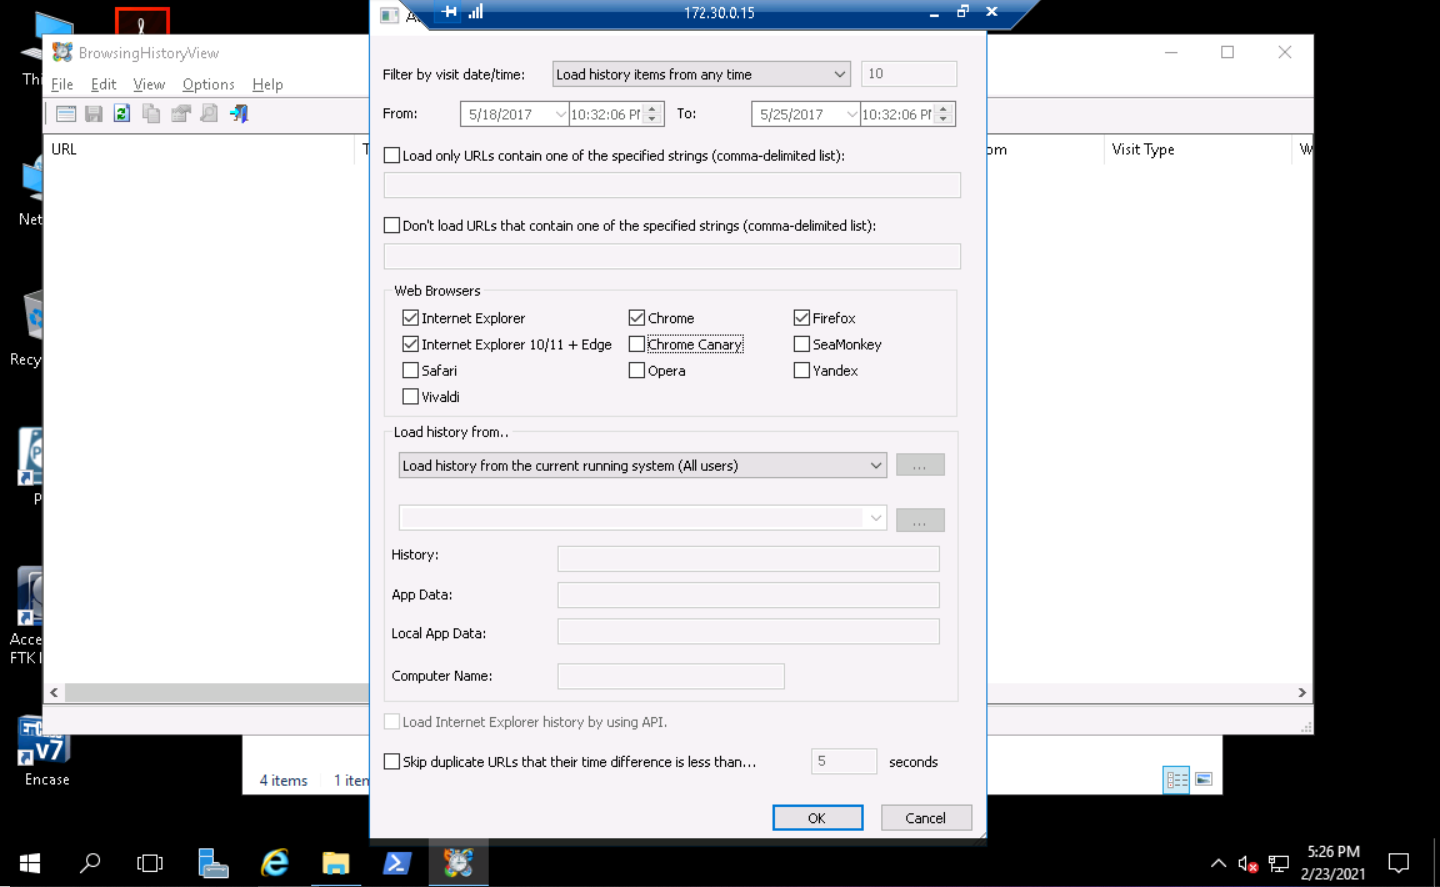
\includegraphics[width=\linewidth]{figures/Part 2 Step 20.png}
    \caption{BrowsingHistoryView list of browsers.}
\end{figure}

\begin{figure}[H]
    \centering
    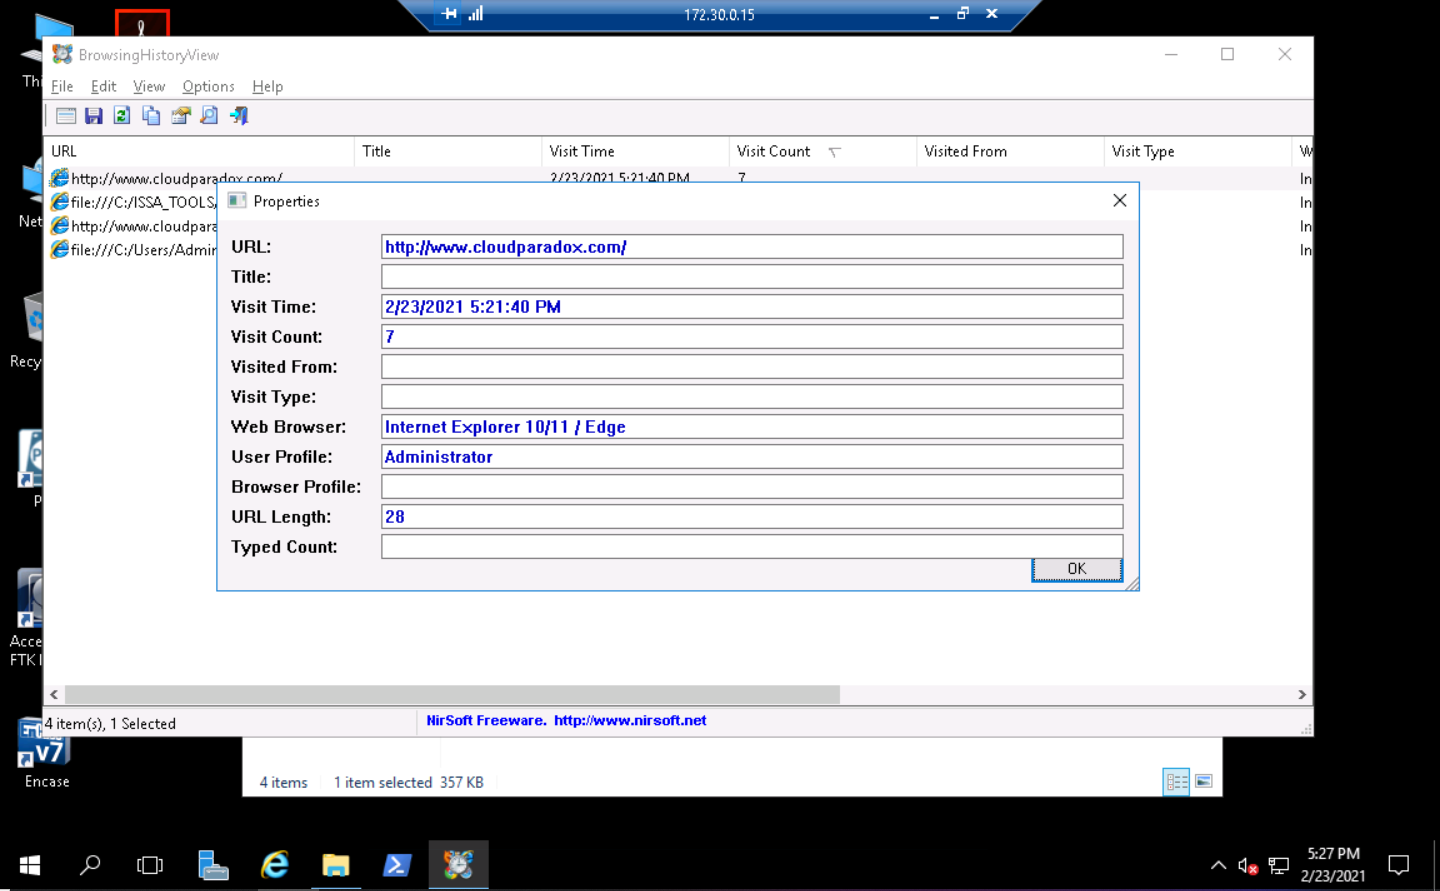
\includegraphics[width=\linewidth]{figures/Part 2 Step 22.png}
    \caption{Properties dialog for CloudParadox Blog.}
\end{figure}

MyLastSearch collects internet search queries made by users using different search engines.
\begin{figure}[H]
    \centering
    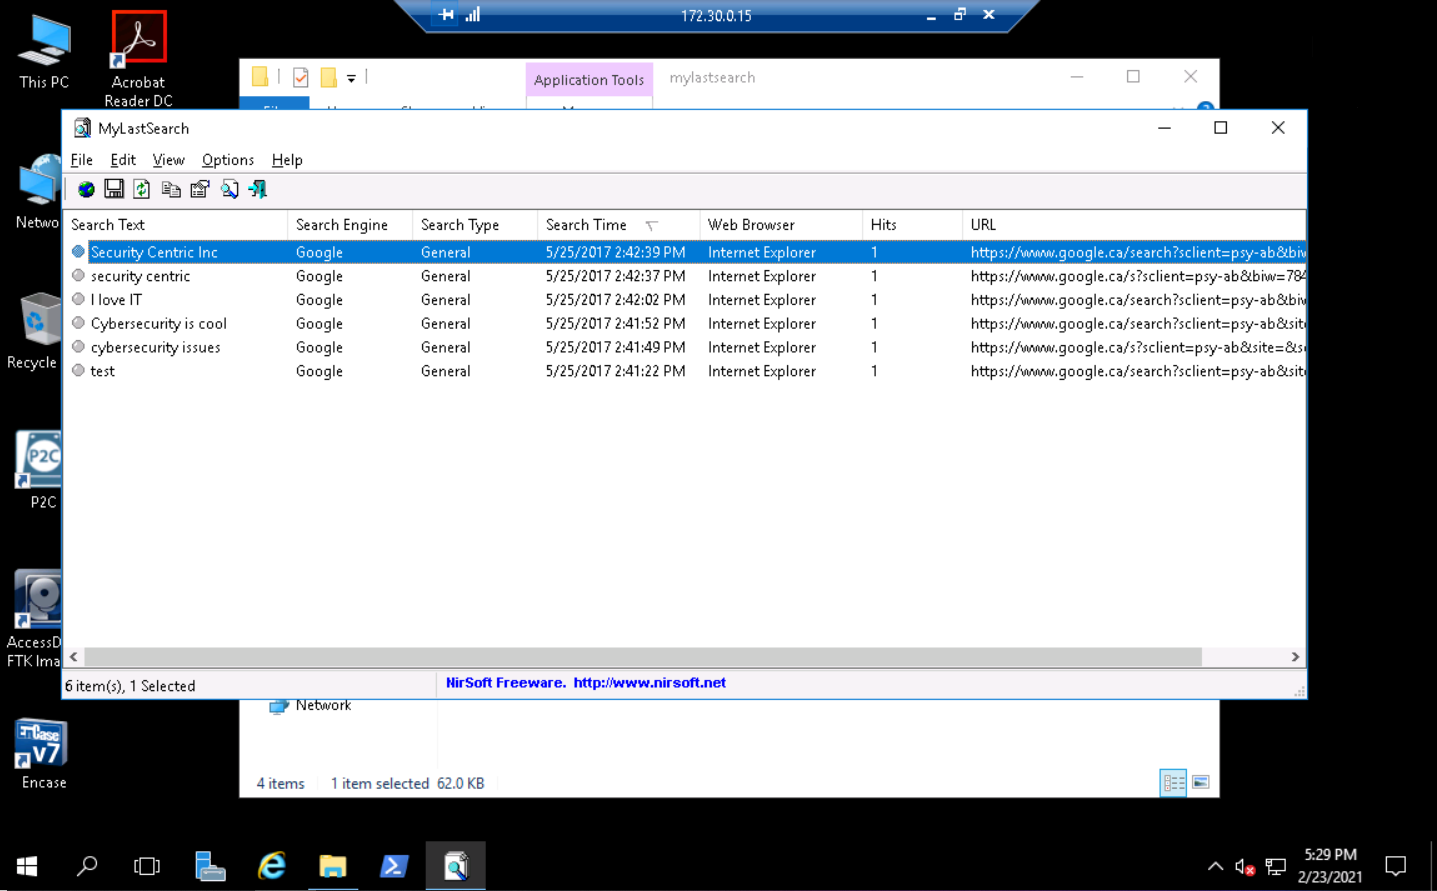
\includegraphics[width=\linewidth]{figures/Part 2 Step 25.png}
    \caption{List of searches with the most recent highlighted.}
\end{figure}

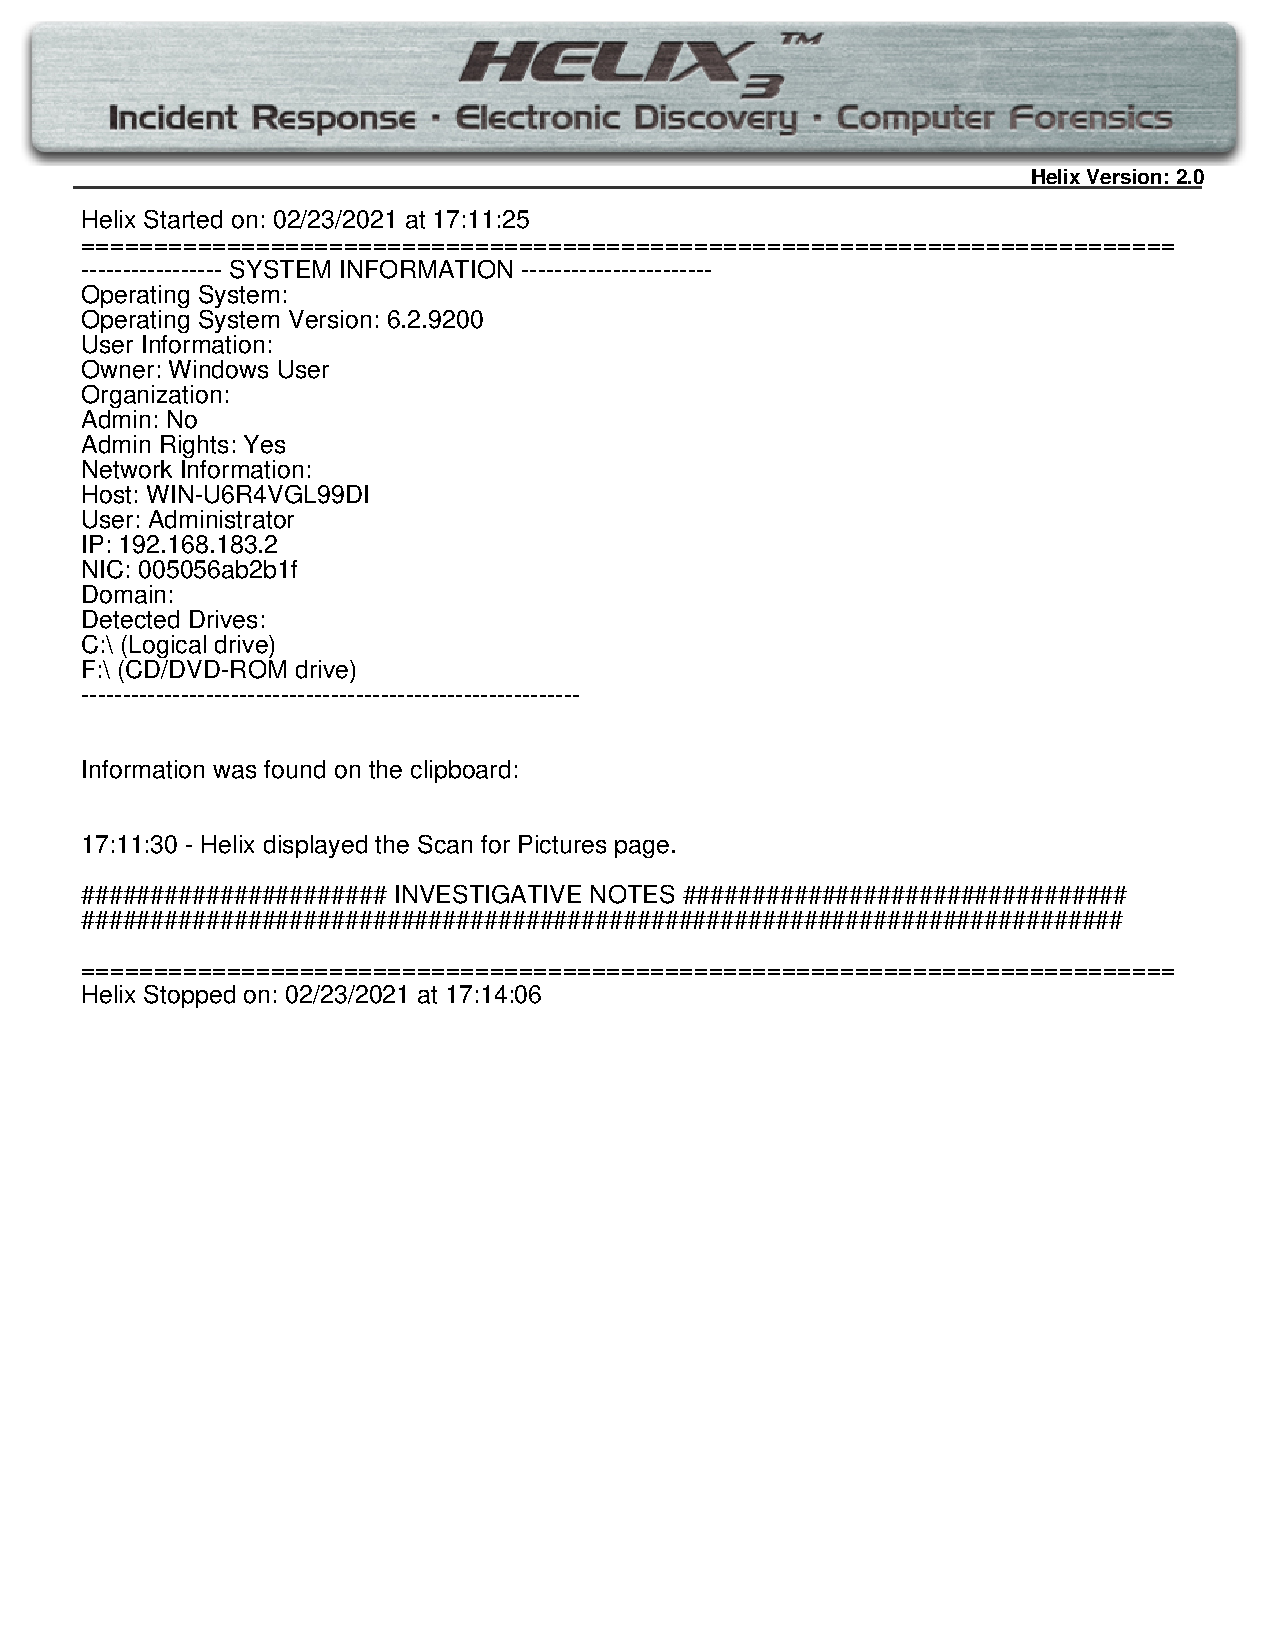
\includepdf[pages=-]{figures/GabrielaAlor_S2_HelixAudit.pdf}

Forensic analysts face challenges of retrieving data from a system without altering evidence in the process.
Using bootable tools means that the host OS is not altered by running these tools.
The tools we used were designed without write capabilities to remove the risk of altering data during retrieval.
During the lab we used the Helix tool to gather in depth information about data on a machine.
Multiple tools were used to gather internet browsing activity such as search history, bookmarks and favorites.